%%
%% This is file `critical_literature.tex',
%%
The loading applied to structures due to an accidental or intentional blast are complex and based on a number of factors (peak pressure, peak  impulse, positive phase duration etc.).  There have been several models developed to predict these factors however, the most common are the Kingery Bulmash (KB) equations \cite{Kingery1984}.  The KB equations are based upon the explosive trinitrotoluene (TNT).  TNT is an explosive with a negative oxygen balance of approximately $-74\%$.  There have been a number of studies that have indicated the role oxygen balance may have on explosive performance.  This literature review will examine some of these studies beginning with an introduction to oxygen balance.

\section{Oxygen Balance}
Oxygen balance is the ratio of the amount of oxygen in an explosive molecule compared with the amount of oxygen required for complete oxidation of the explosive products.  There are three possible oxygen balance outcomes:
\begin{itemize}
\item negative oxygen balance - there is insufficient oxygen for complete oxidation of the explosive products,
\item oxygen balanced - there is exactly enough oxygen for complete oxidation of the explosive products,
\item positive oxygen balance - there is excess oxygen for complete oxidation of the explosive products
\end{itemize}
There are two methods for calculating the oxygen balance.  The first method involves calculating the stoichiometric reaction of the decomposition of the explosive.  If we consider the detonation of TNT, see Figure \ref{fig:tnt}, the reaction results in oxidized gaseous products.  If we assume the products fully react forming carbon dioxide, water, and nitrogen we have,
\begin{equation}\label{eq:tnt_1}
C_7H_5N_3O_6 \rightarrow nCO_2+nH_2O+nN_2
\end{equation}
From the TNT molecule we know there are $7$ moles of carbon, $5$ moles of hydrogen, and $3$ moles of nitrogen in the reactants,
\begin{equation}\label{eq:tnt_2}
C_7H_5N_3O_6 \rightarrow 7CO_2+2\frac{1}{2}H_2O+1\frac{1}{2}N_2
\end{equation}
There are $6$ moles of oxygen in the TNT molecule.  There are $16\frac{1}{2}$ moles of oxygen in the reactants.  Therefore, to balance the equation we need to subtract $10\frac{1}{2}$ moles of oxygen from the reactants,
\begin{equation}\label{eq:tnt_3}
C_7H_5N_3O_6 \rightarrow 7CO_2+2\frac{1}{2}H_2O+1\frac{1}{2}N_2-10\frac{1}{2}O
\end{equation}
This clearly shows that there is insufficient oxygen in the TNT molecule to oxidize all the reactants into water and carbon dioxide.  Oxygen balance is calculated by weight.  The molecular weight $(MW)$ of the TNT molecule is given by,
\begin{figure}
  \begin{center}
   \includegraphics[width=2.0in]{/Users/skmcneill/Documents/Github/comprehensive/5_reports/figures/2019-03-29_tnt_ring.png}
  \end{center}
  \caption{Trinitrotoluene, TNT, $C_7H_5N_3O_6$}
\label{fig:tnt}
\end{figure}%
\begin{equation}\label{eq:tnt_mw1}
MW_{TNT} = 7MW_{C}+5MW_{H}+3MW_{N}+6MW_{O}
\end{equation}
\begin{equation}\label{eq:tnt_mw2}
MW_{TNT} = 7(12.0107)+5(1.00794)+3(14.00674)+6(15.9994)
\end{equation}
\begin{equation}\label{eq:tnt_mw3}
MW_{TNT} = 227.1312
\end{equation}
The molecular weight of the additional oxygen needed is,
\begin{equation}\label{eq:tnt_mw4}
MW_{oxygen} = -10\frac{1}{2}(15.9994)
\end{equation}
\begin{equation}\label{eq:tnt_mw5}
MW_{oxygen} = -167.9937
\end{equation}
Therefore, the oxygen balance is,
\begin{equation}\label{eq:tnt_ob1}
OB\%_{TNT} = \frac{-167.9937}{227.1312}100\%
\end{equation}
\begin{equation}\label{eq:tnt_ob2}
OB\%_{TNT} = -73.96\%
\end{equation}
The second method of calculating oxygen balance is shown in equation \ref{eq:ob1}.  This is only valid for explosives with the form $C_aH_bN_cO_d$.
\begin{equation}\label{eq:ob1}
OB\% = \frac{1599.940\left(d-\left(2a\right)-\left(\frac{b}{2}\right)\right)}{MW}
\end{equation}
where $MW$ is given by,
\begin{equation}\label{eq:ob2}
MW = a(12.0107)+b(1.00794)+c(14.00674)+d(15.9994)
\end{equation}
For nitroglycerin, see Figure \ref{fig:ng}, we have,
\begin{figure}
  \begin{center}
   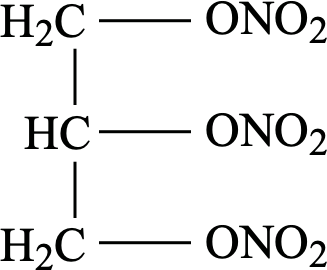
\includegraphics[width=1.1in]{/Users/skmcneill/Documents/Github/comprehensive/5_reports/figures/2019-03-29_ng.png}
  \end{center}
  \caption{Nitroglycerine, NG, $C_3H_5N_3O_9$}
\label{fig:ng}
\end{figure}%
\begin{equation}\label{eq:ng1}
a = 3,\:b = 5,\:c = 3,\:d = 9
\end{equation}
\begin{equation}\label{eq:ng2}
MW_{NG} = 3(12.0107)+5(1.00794)+3(14.00674)+9(15.9994)
\end{equation}
\begin{equation}\label{eq:ng3}
MW_{NG} = 227.094
\end{equation}
Substituting we have,
\begin{equation}\label{eq:ng4}
OB\%_{NG} = \frac{1599.940\left(9-\left(2(3)\right)-\left(\frac{5}{2}\right)\right)}{227.094}
\end{equation}
\begin{equation}\label{eq:ng4}
OB\%_{NG} = 3.52\%
\end{equation}
This indicates that the decomposition of nitroglycerine has a slight positive oxygen balance.  The oxygen balance of several common explosives is summarized in Table \ref{t1} for comparison.
\begin{table}[!h]
\centering
\begin{tabular}{|l|c|r|}
\hline
Explosive        & Empirical Formula     & Oxygen Balance \\
\hline \hline
Ammonium Nitrate & $NH_3HO_3$            & +19.99         \\
\hline
Nitroglycerine   & $C_3H_5N_3O_9$      & +3.52          \\
\hline
PETN             & $C_5H_8N_4O_{12}$ & -10.12         \\
\hline
RDX              & $C_3H_6N_6O_6$      & -21.61         \\
\hline
TNT              & $C_7H_5N_3O_6$      & -73.96         \\
\hline
\end{tabular}
\caption{Oxygen Balance of Some Common Explosives}
\label{t1}
\end{table}


\section{Heat of Detonation}

Decomposition reactions of explosives release energy in the form of heat.  Under adiabatic conditions the release of heat is called the heat of detonation, designated $\Delta H^0_d$.  The heat of detonation is limited to the decomposition of the explosive and does not include any additional heat generated as the products of reaction mix with air.  The heat of detonation indicates the amount of work an explosive can generate as it expands.
The heat of detonation can be calculated from the difference between the heats of formation of the reaction products and the explosive as shown in Equation \ref{eq:Hr}.
 \begin{equation}\label{eq:Hr}
\Delta H^0_r = \sum \Delta H^0_f(reaction\: products) - \Delta H^0_f(explosive)
\end{equation}
where $H^0_f$ is the heat of formation.  The heat of formation is the change in enthalpy associated with the formation of one mole of a compound from its elements in their standard states.  Where the standard state is $25^{\circ} C\:(77^{\circ} F)$ and $101.3\:kPa\:(14.7\:psi)$.  By definition the standard heat of formation of an element is zero. For example, the standard heats of formation of $H_2$, $N_2$, $O_2$ (diatomic elements) is zero, as is the graphite form of solid carbon.

 From \ref{eq:Hr} we can see that the heat of detonation is sensitive to the reaction products and therefore the reaction hierarchy.  Typical examples of reaction hierarchies are the Kistiskowsky-Wilsion Rules ($OB\%>-40$), Modified Kistiakowsky-Wilson Rules ($OB\%<-40$), Springall Roberts Rules, and Kamlet and Jacob Rules \cite{Akhavan:2004fk} \cite{Kamlet1968b}. These rules each generate different products of reaction, but overall are a good approximation and are easy to calculate.  See Tables \ref{k-w_rules}, \ref{m-k-w_rules}, \ref{s-r_rules} and \ref{k-j_rules} for a summary of these rules.
\begin{table}[!h]
\centering
\begin{tabular}{|l|p{12cm}|}
\hline
Step No.       & Reaction Point \\
\hline \hline
1 & Carbon atoms are converted to carbon dioxide, $CO_2$         \\
\hline
2 & If any oxygen remains then hydrogen is oxidized to water, $H_2O$          \\
\hline
3 & If any oxygen still remains then carbon monoxide is oxidized, $CO$         \\
\hline
4 & All the nitrogen is converted to nitrogen gas, $N_2$          \\
\hline
\end{tabular}
\caption{Kistiakowsky-Wilson Rules}
\label{k-w_rules}
\end{table}

\begin{table}[!h]
\centering
\begin{tabular}{|l|p{12cm}|}
\hline
Step No.       & Reaction Point \\
\hline \hline
1 & Hydrogen atoms are converted to water, $H_2O$         \\
\hline
2 & If any oxygen remains then carbon is converted to carbon monoxide, $CO$          \\
\hline
3 & If any oxygen still remains then carbon monoxide is converted to carbon dioxide, $CO_2$         \\
\hline
4 & All the nitrogen is converted to nitrogen gas, $N_2$          \\
\hline
\end{tabular}
\caption{Modified Kistiakowsky-Wilson Rules}
\label{m-k-w_rules}
\end{table}

\begin{table}[!h]
\centering
\begin{tabular}{|l|p{12cm}|}
\hline
Step No.       & Reaction Point \\
\hline \hline
1 & Carbon atoms are converted to carbon monoxide, $CO$         \\
\hline
2 & If any oxygen remains then hydrogen is then oxidized to water, $H_2O$          \\
\hline
3 & If any oxygen still remains then carbon monoxide is oxidized to carbon dioxide, $CO_2$         \\
\hline
4 & All the nitrogen is converted to nitrogen gas, $N_2$          \\
\hline
5 & One third of the carbon monoxide formed is converted to carbon and carbon dioxide, $C$ and $CO_2$          \\
\hline
6 & One sixth of the original amount of carbon monoxide is converted to form carbon and water, $C$ and $H_2O$          \\
\hline
\end{tabular}
\caption{Springall Roberts Rules}
\label{s-r_rules}
\end{table}

\begin{table}[!h]
\centering
\begin{tabular}{|l|p{12cm}|}
\hline
Step No.       & Reaction Point \\
\hline \hline
1 & All nitrogen is converted to nitrogen gas, $N_2$         \\
\hline
2 & Hydrogen atoms are oxidized to water, $H_2O$          \\
\hline
3 & If any oxygen still remains then carbon is oxidized to carbon dioxide, $CO_2$         \\
\hline
4 & All remaining carbon is converted to solid carbon, $C$          \\
\hline
\end{tabular}
\caption{Kamlet Jacobs Rules}
\label{k-j_rules}
\end{table}

For example, if we consider the detonation of TNT using the Springall Roberts Rules we have,

Heat of formation of TNT: $\Delta H^0_f(TNT) = -929.34\:\frac{kJ}{mol}$
Heat

When an explosive has a negative oxygen balance, like TNT, the unoxidized products of reaction are available to react with the oxygen in the air in a combustion reaction called afterburn.  In many cases the afterburn reaction can release more energy than the heat of detonation.  The next section will detail the calculation of the heat of afterburn.
\section{Heat of Afterburn}

\section{Introduction to Shockwaves}
A shockwave is a pressure disturbance moving through a medium faster than the speed of sound with a sharp increase in pressure, density, and temperature.  The disturbance is typically caused by a mechanical event (supersonic bullet), electrical event (a lightening strike), or a chemical event (detonation of an explosive).  When an explosive is detonated the shockwave is commonly referred to as a detonation wave or blast wave.  A blast wave is sustained by the chemical energy of the detonation, however the wave is also losing energy as it propagates due to viscous effects.  Without a continuous supply of  chemical energy to propel the blast wave forward it will eventually dissipate to a sound wave.

\subsection{Basic Shockwave Equations}
The shockwave shown in Figure \ref{fig:sw_cons} was first described mathematically by Rankine and Hugoniot \cite{Rankine1870}\cite{Hugoniot1889}\cite{johnson1998}.  The now called Rankine-Hugonoit jump equations are based on the conservation of mass, momentum, and energy, see Figure \ref{fig:sw_cons}.  The equations are based on the following assumptions:
\begin{itemize}
\item 1D flow,
\item discontinuous shock,
\item transport effects (mass, energy, charge, momentum and angular momentum) out of the system are ignored,
\item reaction rate is instantaneous and complete, and
\item the shock is in steady-state condition before and after the shock.
\end{itemize}
The equations for a detonation wave with the coordinate system fixed to the shockwave are given by,

\noindent
conservation of mass: 
\begin{equation}\label{eq:conservation_of_mass1}
\rho_0 (U - u_0) = \rho_1(U - u_1)
\end{equation}
conservation of momentum: 
\begin{equation}\label{eq:conservation_of_momentum}
P_0 + \rho_0 u_0^2 = P_1 + \rho_1 u_1^2
\end{equation}
conservation of energy: 
\begin{equation}\label{eq:conservation_of_energy}
e_0 + P_0\nu_0 + \frac{1}{2}\left(U-u_0\right)^2 = e_1 + P_1\nu_1 + \frac{1}{2}\left(U - u_1\right)^2
\end{equation}

\begin{figure}
  \begin{center}
   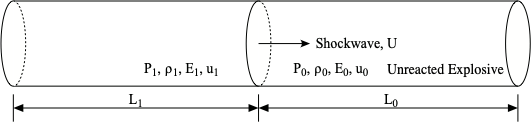
\includegraphics[width=5in]{/Users/skmcneill/Documents/Github/comprehensive/5_reports/figures/conservation_shockfront.png}
  \end{center}
  \caption{Motion of a shockwave showing the discontinuous jump in pressure, temperature, and density.}
\label{fig:sw_cons}
\end{figure}%

\noindent
Where $\rho$ is the density, $P$ is the pressure, $u$ is the particle velocity, $U$ is the shock velocity, $e$ specific energy and the subscripts $0$ and $1$ refer to the reactant and product states, respectively. Unfortunately, these three equations are insufficient to solve for the five unknowns.  Equations of state are needed to provide the additional equations.  Three empirically-derived equations-of-state were developed between the following parameters \cite{March1980}\cite{Cooper1996}:
\begin{itemize}
\item shock velocity and particle velocity $U-u$ plane
\item pressure and specific volume, $P-\nu$ plane
\item pressure and particle velocity, $P-u$ plane
\end{itemize}
These relationships provide a fourth set of equations and are specific to the material (inert or explosive) undergoing a shock and are referred to collectively as Hugoniot equations, see Figure \ref{fig:hugoniot}.  These relationships represent the possible states of the material both pre and post-shock.  For inert materials there is only a single Hugoniot curve but for explosives there is a reactants curve and a products curve, see Figure \ref{fig:hugoniot_inert_explosive}.  These equations consider the products of reaction to be uniform i.e. no individual chemical species present.

 \begin{figure}
  \begin{center}
   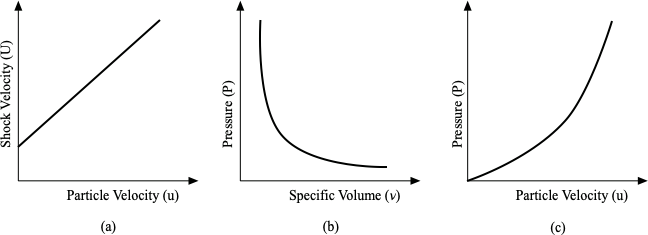
\includegraphics[width=5in]{/Users/skmcneill/Documents/Github/comprehensive/5_reports/figures/hugoniot_example_plots.png}
  \end{center}
  \caption{Typical plots of (a) the $U-u$ plane, (b) the $P-\nu$ plane, and (c) the $P-u$ plane.  These curves were developed experimentally using standard curve-fit techniques.}
\label{fig:hugoniot}
\end{figure}%
  
 \begin{figure}
  \begin{center}
   \includegraphics[width=5in]{/Users/skmcneill/Documents/Github/comprehensive/5_reports/figures/hugoniot_reactive_unreactive.png}
  \end{center}
  \caption{ $P\mbox{-}\nu$ plane showing (a) an example of an inert material transitioning from state (0) pre-shock to state (1) post-shock (b) and an example of an explosive transitioning from the unreacted Hugoniot (0) pre-shock to the detonation products Hugoniot (1') post-shock.  Note the unreacted explosive Hugoniot in (b) also transitions to state (1).  Point (1) represents the explosive just prior to detonation.  The line connecting the initial and final states is called the Raleigh line.}
\label{fig:hugoniot_inert_explosive}
\end{figure}%

In the $P\mbox{-}\nu$ plane, the line connecting the initial (0) and final (1) states in Figure \ref{fig:hugoniot_inert_explosive} is a jump condition.  This line is called the Raleigh line.  Recalling the conservation of mass and momentum equations and that $\nu = 1/\rho$,

\begin{equation}\label{eq:mass}
\frac{u_0}{\nu_0} = \frac{u_1}{\nu_1} = \frac{\nu_0}{\nu_1} = \frac{u_0}{u_1}
\end{equation}

\begin{equation}\label{eq:momentum}
p = P_0 + \rho_0 u_0^2 = P_1 + \rho_1 u_1^2
\end{equation}and assuming $u_0=0$ we can rewrite equation \ref{eq:mass},
\begin{equation} \label{eq:u1}
u_1=\frac{u_0(\nu_1)}{\nu_0}
\end{equation}
Substituting equation \ref{eq:u1} into equation \ref{eq:momentum} and performing some algebra we have,
\begin{equation}
P_1-P_0=-\frac{U^2}{\nu_0^2}\left(\nu_1-\nu_0\right)
\end{equation}
Recalling that the equation for a line is given by,
\begin{equation}
y_1-y_0 = m(x_1-x_0)
\end{equation}
where $m$ is the slope of the line then the slope of the Raleigh line in the $P-\nu$ plane is,
\begin{equation}
m = -\frac{U^2}{\nu_0^2}
\end{equation}
or, 
\begin{equation} \label{eq:shock_velocity}
U = -\rho_0m^{1/2}
\end{equation}

	
The empirically derived Hugoniot equations combined with the mass, momentum, and energy equations are successful in solving a range of shock related problems.  Typical problems include:
\begin{itemize}
\item material impact problems
\item shockwave behavior between materials with different impedances
\item colliding shockwave behavior
\end{itemize}

\subsection{Reactive Shockwaves}
In the previous discussion, the reaction rate behind the shockwave was considered instantaneous.  If we wish to consider a finite reaction rate we can use the Zeldovich-von Neumann-Doering (ZND) model\cite{Zeldovich1940}\cite{VonN1942}.  The assumptions for the reactive shockwave are as follows:
\begin{itemize}
\item 1D flow,
\item Discontinuous shock (transport effects neglected),
\item Reaction rate is zero at the shock and finite behind the shock and the reaction is irreversible,
\item Thermodynamics are at equilibrium except in the reaction zone.
\end{itemize}
In this model, the shockwave discontinuity is replaced with a shockwave and a finite reaction zone.  The initial state in front of the shockwave remains unchanged however, the final state is now the end of the reaction zone, see Figure \ref{fig:p_t_reaction_zone}. 
 \begin{figure}
  \begin{center}
   \includegraphics[width=5in]{/Users/skmcneill/Documents/Github/comprehensive/5_reports/figures/conservation_reactive_shockfront.png}
  \end{center}
  \caption{Shockwave with a reaction zone ranging from no reaction $\lambda_0$ to reaction complete $\lambda_1$.}
\label{fig:p_t_reaction_zone}
\end{figure}%
The mass and momentum equations across the reactive shock are the same as for the basic shockwave, equations  \ref{eq:conservation_of_mass1} and \ref{eq:conservation_of_momentum}.  The energy equation however, depends on the degree of chemical reaction $\lambda$.  Where $\lambda$ varies from 0 (no reaction) to 1 (reaction complete).  The energy from chemical reaction appears in the internal energy term $e$ in the conservation of energy equation,
\begin{equation}\label{eq:conservation_of_energy_reactive}
e_1 \lambda_1-e_0 \lambda_0=\frac{P_1u_1-P_0-u_0}{\rho_0(U-u_0)}-\frac{1}{2}(u_1^2-u_0^2)
\end{equation}
If an equation of state is known (same requirement as the basic shockwave equation) and a reaction rate equation is known we can calculate the thermodynamic properties inside the reaction zone as a function of time or distance.  If we consider the $P\mbox{-}\nu$ plane again, we would have multiple Hugoniot curves as the reaction goes to completion, see Figure \ref{fig:zdn_reaction_zone}. However, even simple reaction rate equations that produce plausible results require numeric analysis.
 \begin{figure}
  \begin{center}
   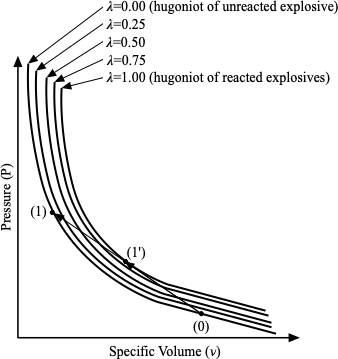
\includegraphics[width=3.5in]{/Users/skmcneill/Documents/Github/comprehensive/5_reports/figures/hugoniot_znd_plots.png}
  \end{center}
  \caption{Family of Hugoniot curves related to successive quarters of reacted, $\lambda$, explosive.}
\label{fig:zdn_reaction_zone}
\end{figure}%

\subsubsection{Oxygene Balance}
\lipsum[10]
\subsubsection{Heat of Explosion}
\lipsum[10]
\subsubsection{Heat of Afterburn}
\lipsum[10]

\section{Air Blast Parameters}
\lipsum[10]
\subsection{Kingery and Pannill - 1964}
\lipsum[10]
\subsection{Kingery - 1966}
\lipsum[10]
\subsection{Kingery and Bulmash - 1984}
\lipsum[10]
\subsection{Polynomial Equations for Airblast Parameters at Small Scaled Distances}
\lipsum[10]
\subsection{Measuring Air Blast}
\lipsum[10]
\subsection{Measuring Fireball Temperature}
\lipsum[10]

\section{Blast Resistant Design}
\lipsum[10]

\endinput
%%
%% End of file `critical_literature.tex'.
